\chapter{Background} 
\label{c:Background}
The goal of the paper \textit{\acrshort{snh}} was to simulate the fleshy appearance of virtual characters. In order to follow their thought process, we first need to understand the physical and mathematical interpretation of a deformation. This chapter serves as an introduction into the field of continuum mechanics and describes the mathematical background needed to understand the calculations and conclusions. At the beginning of this chapter, I will define the notation that I will use throughout this whole thesis. Next, I will present some concepts used in continuum mechanics, which are crucial for this field. Thirdly, I will give some insights into the mathematics used in continuum mechanics. However, I will not include each proof explicitly, as there are already many resources for an interested reader. Finally, I will introduce a few calculations and conclusions that will be useful to understand the methods used in the paper \textit{\acrshort{snh}}.

\section{Notation}
This section defines the notation that is used throughout this thesis to avoid misunderstandings. I am using the common notation used in continuum mechanics taken from the book \textit{Continuum Mechanics} (\cite{Spencer1980}). Additionally, I am including some more specific declarations formulated and used by the authors of the paper \textit{\acrshort{snh}}.

\subsection{General Notation}
Scalars are represented by regular, normal-weight variables such as $a$, whereas tensors and matrices are represented by upper-case bold letters, such as $\textbf{A}$. Vectors will be denoted by bold lower-case variables like $\textbf{a}$. 

\subsection{Tensor Notation}
Furthermore, I am using the tensor notation used in \textit{\acrshort{snh}}. Similar to Golub and Van Loan (\cite{golub2012matrix}), the authors decided to define the vectorization vec(\cdot) as column-wise flattening of a matrix into a vector:
\[
\mathbf{A} = \begin{bmatrix} a & c \\ b & d \end{bmatrix} \qquad \operatorname{vec}(\mathbf{A}) = \begin{bmatrix} a \\ b \\ c \\ d \end{bmatrix}
\]
Additionally, $4^{th}$ order tensors in a form of matrix-of-matrices will be used in the calculations in \autoref{c:Paper}. These matrices are denoted by using blackboard bold:
\[
\mathbb{A} = 
\left[\begin{array}{cc}{\begin{bmatrix} a & c \\ b & d \end{bmatrix}} & {\begin{bmatrix} i & k \\ j & l \end{bmatrix}} \\ {\begin{bmatrix} e & g \\ f & h \end{bmatrix}} & {\begin{bmatrix} m & o \\ n & p \end{bmatrix}}\end{array}\right]
=
\left[\begin{array}{cc}{\left[\mathbf{A}_{00}\right]} & {\left[\mathbf{A}_{01}\right]} \\ {\left[\mathbf{A}_{10}\right]} & {\left[\mathbf{A}_{11}\right]}\end{array}\right]
\]
By vectorizing $\mathbb{A}$ we get the following result:
\[
\operatorname{vec}(\mathbb{A}) = \left[ \,\operatorname{vec}\left(\mathbf{A}_{00}\right)\, \bigg| \,\operatorname{vec}\left(\mathbf{A}_{10}\right)\, \bigg| \,\operatorname{vec}\left(\mathbf{A}_{01}\right)\, \bigg| \,\operatorname{vec}\left(\mathbf{A}_{11}\right)\, \right] = \mathbf{\check{A}}
\]
In order to point out that a matrix is vectorized, I am using the symbol $\check{\cdot}$ above the letter. The term above is equivalent to
\[
\mathbf{\check{A}}=\left[\begin{array}{llll}{a} & {e} & {i} & {m} \\ {b} & {f} & {j} & {n} \\ {c} & {g} & {k} & {o} \\ {d} & {h} & {l} & {p}\end{array}\right].
\]
The advantage of this form is that we can write several expressions as a cross product. This property will be used in \autoref{c:Paper} to simplify complicated expressions and calculations.

\subsection{Summary}
Here is a quick overview of the introduced notation:
\begin{align*}
a&: \text{Scalar} \\
\mathbf{A}&: \text{Matrix or tensor} \\
\mathbf{a}&: \text{Vector} \\
\mathbb{A}&: \text{Matrix-of-matrices} \\
\mathbf{\check{A}}&: \text{Vectorized matrix-of-matrices (also written as vec($\mathbb{A}$))}
\end{align*}

\section{Concepts of Continuum Mechanics}
This section gives a broad introduction to some of the concepts used in continuum mechanics. In continuum mechanics, we are less interested in small particles like atoms or molecules of an object but rather in pieces of matter that are large in comparison. The reason for this is that the calculation for the behaviour of individual atoms is challenging for larger systems. Therefore, we are concerned with the mechanical behaviour of solids and fluids on the macroscopic scale and treat the material as uniformly distributed throughout regions of space. With this approach, it is possible to define quantities such as displacement and density as continuous functions of the position (\cite{Spencer1980}, p. 1).

\subsection{Deformation}
When studying an object, we are among other properties interested in how it may change its shape over a certain period of time. If the object undergoes a change of shape, we call this process a deformation. In order to produce a deformation, there must be at least one force present that interacts with the object. Typically, we apply one or multiple forces over an object and are then interested in its deformed state. The term \textit{strain} is used as a measure of deformation, and we denote \textit{stress} as the force per unit area. 

Graphically, we can imagine a deformation with the help of a two-dimensional deformation map, as shown in Fig. \ref{fig:deformationmap}. The ellipse on the left side represents an object in its rest state. A function $\phi$ maps this rest state of the ellipse to a deformed state as shown on the right side of the image.
\begin{figure}[!htbp]
	\centering
	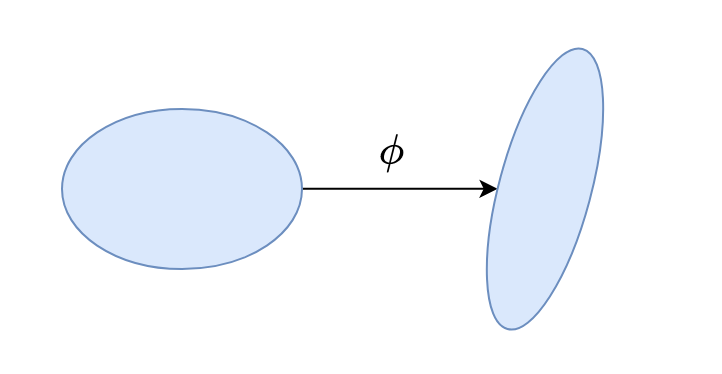
\includegraphics[width=0.6\textwidth]{resources/deformation_map_plain.png}
	\caption[Deformation Map]{Deformation Map}
	\label{fig:deformationmap}
\end{figure}

We can imagine that we map each particle of a chosen object from its rest state to a deformed one. We can characterize each particle $X$ of a body by a vector $\mathbf{x}$ containing its positional coordinates. This vector is the reference configuration. If we displace the particle, we can describe its new coordinate vector $\mathbf{x}'$ with 
\[
	\mathbf{x}' = \phi (\mathbf{x}).
\]
\textbf{\textit{Example:}} A simple example of a deformation is the stretching of a cuboid along the x- and y-axis, as illustrated in Fig. \ref{stretch:1}. 
\begin{figure}[!htbp]
	\centering
	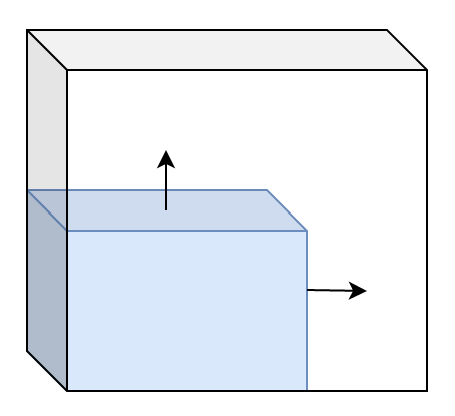
\includegraphics[width=0.35\textwidth]{resources/stretch_plot_new.png}
	\caption[Stretching of a cuboid]{Stretching of a cuboid}
	\label{stretch:1}
\end{figure}

The coloured volume in Fig. \ref{stretch:1} represents the cuboid in its rest state. In this case, the vector $\mathbf{x}$ contains the three coordinate values for the x-, y-, and z-axis:
\[
	\mathbf{x} = \begin{bmatrix} x \\ y \\ z\end{bmatrix}
\]
After the stretching, the new position for each particle can be calculated by
\begin{equation} \label{eq:example_phi}
	\mathbf{x}' = \phi (\mathbf{x}) = \begin{bmatrix} 1.5x + 0y + 0z	 \\ 0x + 2y + 0z \\ 0x +0y + 1z \end{bmatrix} = \begin{bmatrix} 1.5x \\ 2y \\ z \end{bmatrix}.
\end{equation}

\subsection{Deformation Gradient}
\label{ss:deformation_gradient}
An essential quantity in continuum mechanics is the deformation gradient \textbf{F}. It serves as a characterization of the deformation. With its help, we can calculate properties like the change of volume or length of an object during a deformation. We can obtain \textbf{F} by using the function $\phi$ discussed in the previous section and taking the derivative of each component of $\phi$ with respect to each component of the reference vector \textbf{x}. In the following, we only work with deformations in the three-dimensional space. In that case, $\mathbf{F}$ is a ($3 \times 3$)-matrix and can be calculated by
\begin{equation}\label{eq:deformation_gradient_general}
\mathbf{F} = \left[ \,\frac{\phi(\mathbf{x})}{\partial x}\, \bigg| \,\frac{\phi(\mathbf{x})}{\partial y}\, \bigg| \,\frac{\phi(\mathbf{x})}{\partial z}\, \right].
\end{equation}
For simplification, I will use this representation of \textbf{F} in the upcoming chapters:
\begin{equation}  \label{eq:deformation_gradient}
\textbf{F} = \left[ \,\mathbf{f_0}\, \bigg| \,\mathbf{f_1}\, \bigg| \,\mathbf{f_2}\, \right] = \begin{bmatrix} f_0 & f_3 & f_6 \\ f_1 & f_4 & f_7 \\ f_2 & f_5 & f_8 \end{bmatrix} 
\end{equation}
In this equation, $\mathbf{f_i}$ are the column vectors, and $f_i$ symbolize the scalar entries of the matrix. \textbf{F} can be useful for us to find out more about the deformation. For example, we know that if \textbf{F} is equal to the identity matrix \textbf{I}, there is no deformation present. That would be the case for rigid body displacements. In addition, \textbf{F} can be factorized and used to calculate other quantities. That will be explained in \autoref{s:deformation_gradient} after introducing the needed theorems in \autoref{s:math_background}.

\textbf{\textit{Example:}} I am again taking the example of stretching the cuboid from Fig. \ref{stretch:1}. We can obtain the resulting deformation gradient of this example with the help of Eq. \eqref{eq:deformation_gradient_general} applied to Eq. \eqref{eq:example_phi}:
\[
	\mathbf{F} = \left[ \,\frac{\phi(\mathbf{x})}{\partial x}\, \bigg| \,\frac{\phi(\mathbf{x})}{\partial y}\, \bigg| \,\frac{\phi(\mathbf{x})}{\partial z}\, \right] 
	= \begin{bmatrix} \frac{\partial [1.5x]}{\partial x} & \frac{\partial [1.5x]}{\partial y} & \frac{\partial [1.5x]}{\partial z} \\ \frac{\partial [2y]}{\partial x} & \frac{\partial [2y]}{\partial y} & \frac{\partial [2y]}{\partial z} \\ \frac{\partial [z]}{\partial x} & \frac{\partial [z]}{\partial y} & \frac{\partial [z]}{\partial z} \end{bmatrix} = \begin{bmatrix} 1.5 & 0.0 & 0.0 \\ 0.0 & 2.0 & 0.0 \\ 0.0 & 0.0 & 1.0 \end{bmatrix}
\]
As we can see, $\mathbf{F}$ is not equal to the identity matrix, so we are sure that the object was indeed deformed. For this simple example, this information might seem unnecessary because the visualisation already shows that the cuboid gets deformed, but for more complex deformations, this information is very useful.

\subsection{Deformation Energy}
\label{ss:deformation_energy}
We can deform an object by putting a certain amount of force into the system. We could, for example, stretch a spring. The spring then stores some amount of potential energy. If we let the spring go, we transfer the potential energy to kinetic energy, and the spring usually recovers into its rest state. This energy that the spring stores during the deformation is called \textit{deformation energy} or \textit{strain energy} $\Psi$. The strain energy density is the strain energy per unit volume. Any increment of the strain energy density is equal to the work done by the stresses in order to alter the strains (\cite{KORSUNSKY20175}, p.10). That means that energy is an indicator of how much force must be applied to deform an object in a certain way. Thus, we can use the deformation energy to express the relationship between the stresses and strains. We can illustrate this with a stress-strain curve shown in Fig. \ref{fig:stress_strain}. The area under the stress-strain curve corresponds to the strain energy density.
\newpage
\begin{figure}[!htbp]
	\centering
	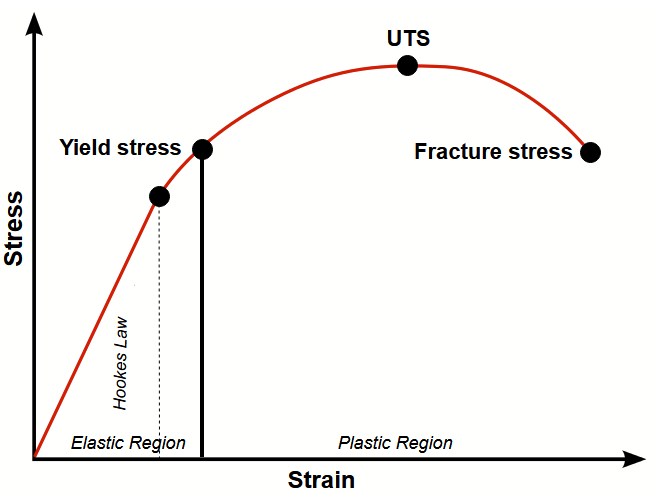
\includegraphics[width=0.7\textwidth]{resources/stress_strain_curve_final.png}
	\caption[Stress-strain curve]{Example for a stress-strain curve\footnotemark}
	\label{fig:stress_strain}
\end{figure}
\footnotetext{the orginial image was taken from: \newline https://commons.wikimedia.org/wiki/File:Stress-strain\_curve.svg}

As we can see in Fig. \ref{fig:stress_strain}, with increasing stress, the object goes through different states. Before reaching the yielding point illustrated with \textit{Yield stress}, the material has the ability to recover into its rest shape. This ability is called \textit{Elasticity} (\cite{BERGSTROM2015209}, p. 211). After this point, the material cannot recover anymore due to permanent fractures during the deformation.

In addition, we can see that at the beginning of the curve, we have a straight line until the first black dot. That means that the relationship between the stresses and strains is linear. This is called \textit{Linear Elasticity} (\cite{KORSUNSKY20175}, p. 5). Linear elasticity is strictly related to \textit{Hooke's law}, which states that the resulting deformation is proportional to the applied force and that the object is able to recover into its rest shape under these conditions. Hence, we can also say that the material is consistent with \textit{Hooke's law} in this interval.

After the straight line, we can spot a non-linear relationship before the yielding point. The material is still able to recover, but there is a non-linear relationship between the stresses and strains. The resulting deformation is larger than how Hooke's law would predict it. Materials that fall into this category are called \textit{Hyperelastic Materials}. Hyperelasticity is a generalization of linear elasticity with a non-linear relationship and is suited for larger strain predictions (\cite{BERGSTROM2015209}, p. 218).

\textit{\acrshort{uts}} in Fig. \ref{fig:stress_strain} is abbreviated for \acrlong{uts} and defines the maximal stress an object can bear before breaking. At the point of \textit{Fracture stress} the material finally tears apart.

The behaviour of the object depends heavily on the material it consists of, and the stress-strain curve looks different for each material. We need to choose the energy function according to the material properties. The behaviour of human flesh can be put into the category of hyperelastic materials. Thus, the energy function also has to be hyperelastic for our purposes. 

\subsection{Material Constants}
\label{ss:material_constants}
When we look at a deformation of an object, we need to consider the material the object consists of. Materials can be very stiff like steel or easily deformable like rubber. In order to measure the deformation of a specific material, we need the Poisson's ratio of said material. The Poisson's ratio is a material constant that is defined as 
\begin{equation}\label{eq:poisson}
\nu = - \frac{\epsilon_{11}}{\epsilon_{22}} \in [-1, 0.5],
\end{equation}
where $\epsilon_{11}$ is the lateral and $\epsilon_{22}$ the axial strain. The range in which $\nu$ lies in starts at $-1$ and goes up to $0.5$ (\cite{PhysRevB.80.132104}). In order to understand this quantity better, we can use an example: Imagine pulling a rubber band on each of its sides. After pulling a bit, we can observe that the band gets longer and the middle part gets narrower. The Poisson's ratio indicates the extent of this deformation. Some materials, such as rubber, are more easily deformable and therefore lead to a higher Poisson's ratio.

Usually, the Poisson's ratio of a material is positive. A negative value would mean that the material becomes wider in the cross-section when we stretch it. This behaviour is very uncommon in nature. Examples of materials with a negative Poisson's ratio are for instance discussed in \textit{Foam structures with a negative Poisson's ratio} (\cite{lakes1987foam}) or \textit{Advances in negative Poisson's ratio materials} (\cite{lakes1993advances}). Table \ref{table:1} shows examples of positive Poisson's ratios of various materials.

\setlength{\tabcolsep}{0.5em} % for the horizontal padding
{\renewcommand{\arraystretch}{1.1}% for the vertical padding
\begin{table}[!htbp]
\centering
    \begin{tabular}{ | l | l |}
    \hline
    \textbf{Material} & \textbf{Poisson's ratio} \\ \hline
    C (graphite) & 0.31 \\ \hline
    Sn (metal) & 0.357 \\ \hline
    Cu & 0.355 \\ \hline
    Zn & 0.25 \\ \hline
    Ag & 0.36 \\ \hline
    Au & 0.45 \\ \hline
    Concrete & 0.20–0.37 \\ \hline
    Titanium (dental alloy) & 0.30–0.31 \\ \hline
    Bronze & 0.34 \\ \hline
    18–8 Stainless steel & 0.305 \\ \hline
    Natural rubber & 0.4999 \\ \hline
	B\textsubscript{2}O\textsubscript{3} glass & 0.30 \\ \hline
	GeO\textsubscript{2} glass & 0.20 \\ \hline	
    \end{tabular}
    \caption[Materials with their Poisson's ratio]{Different materials with their Poisson's ratio (\cite{PhysRevB.80.132104}, p. 3)}
\label{table:1}
\end{table}

In the context of flesh simulation, the Poisson's ratio tells us how resistant flesh is to volume change. The
Poisson's ratio of biological tissues such as flesh, fat, and muscles takes on higher values in the range of 0.45 and 0.5 (\cite{Smith:2018:SNF:3191713.3180491}).

The calculation of the Poisson's ratio, as defined in Eq. \eqref{eq:poisson}, is a challenge. Fortunately, we can make use of the \textit{Lamé Parameters}, the two material-specific constants $\mu$ and $\lambda$. With the help of these two constants, we can transform Eq. \eqref{eq:poisson} into the form
\begin{equation}\label{eq:poisson_ratio}
\nu =  \frac{\lambda}{2(\lambda + \mu)}.
\end{equation}
This equation allows us to calculate the Poisson's ratio much easier (\cite{BERGSTROM2015209}, p. 231).

\section{Mathematical Background}
\label{s:math_background}
Now that we have established an understanding of the general concepts of continuum mechanics, we can look at the more technical part. Since mathematics play an important role in the field of interests, we need to build a solid background before diving further into more technical calculations. This section covers all the essential concepts used later in the calculations. A basic understanding of linear algebra is assumed.

\subsection{Singular Value Decomposition}
The \acrlong{svd} (\acrshort{svd}) will play an important role while working with the deformation gradient. It represents the best possible approximation of a given matrix by a matrix of low rank. This approximation can be looked at as a compression of the given data (\cite{LiesenMehrmann2015}, p. 295). Firstly, we need to define what singular values are.
\begin{definition}[\textbf{Singular Values}]
\label{singular_values}
The singular values of a matrix $\mathbf{A}$ $\in$ $\mathbb{R}^{m \times n}$ are the square roots of the eigenvalues of $\mathbf{AA}^{\mathsf{T}}$.
\end{definition}
The theorem of the singular value decomposition states that we can factor every ($m \times n$)-matrix into one orthogonal ($m \times m$)-, one orthogonal ($n \times n$)-, and one diagonal ($m \times n$)-matrix. More formally:
\begin{theorem}[\textbf{The \acrshort{svd} Theorem}]
\label{SVD}
Let $\mathbf{A}$ $\in$ $\mathbb{R}^{m \times n}$ be a matrix having r positive singular values, m $\geq$ n. Then there exist orthogonal matrices $\mathbf{U}$ $\in$ $\mathbb{R}^{m \times m}$, $\mathbf{V}$ $\in$ $\mathbb{R}^{n \times n}$ and a diagonal matrix $\mathbf{\tilde{\Sigma}}$ $\in$ $\mathbb{R}^{m \times n}$ such that
\begin{align*}
\mathbf{A} &= \mathbf{U \tilde{\Sigma} V^\mathsf{T}} \\
\mathbf{\tilde{\Sigma}} &= \left[ \begin{array}{cc} \mathbf{\Sigma} & 0 \\ 0 & 0 \end{array} \right]
\end{align*}
where $\mathbf{\Sigma}$ = diag ($\sigma_1$, $\sigma_2$, . . . , $\sigma_r$), and $\sigma_1$ $\geq$ $\sigma_2$ $\geq$ · · · $\geq$ $\sigma_r$ $>$ 0 are the positive singular values of $\mathbf{A}$.
\end{theorem}
This definition and theorem were taken from \textit{Numerical linear algebra with applications: Using MATLAB} (\cite{ford2014numerical}, p. 113, p. 300).

\subsection{Polar Decomposition}
Another theorem I will be using in \autoref{s:deformation_gradient} is the polar decomposition theorem:
\begin{theorem}[\textbf{The Polar Decomposition Theorem}]
\label{PD}
Let $\mathbf{F}$ be a non-singular square matrix. Then $\mathbf{F}$ can be decomposed uniquely into either of the following two products
\[
\mathbf{F} = \mathbf{RU}, \quad \mathbf{F} = \mathbf{VR}
\]
where $\mathbf{R}$ is an orthogonal matrix, and $\mathbf{U}$ and $\mathbf{V}$ are positive definite symmetric matrices.
\end{theorem}

This theorem was taken from \textit{Continuum Mechanics}, in which they include the proof for ($3 \times 3$)-matrices (\cite{Spencer1980}, p. 12).

\subsection{Frobenius Norm}
The Frobenius norm is a matrix norm. It allows us to measure and compare entities in a multidimensional space.
\begin{definition}[\textbf{Frobenius Norm}]
\label{FN}
Let \textbf{A} be an (m $\times$ n)-matrix in the real or complex domain. Then the Frobenius norm is defined as 
\[
\| \mathbf{A} \|_{F} := \sqrt{\sum\limits_{i=1}^{m} \sum\limits_{j=1}^{n} |a_{ij}|^2}.
\]
\end{definition}
We can further represent the norm with the trace of the matrix, in which $\mathbf{A}^*$ is the conjugate transpose of \textbf{A}. We can then use the \acrshort{svd} of \textbf{A} and write the norm with respect to the singular values of \textbf{A}, denoted by $\sigma_i$:
\begin{equation} \label{eq:FN}
\| \mathbf{A} \|_{F} = \sqrt{\operatorname{trace}(\mathbf{A} \mathbf{A}^*)} = \sqrt{\sum\limits_{i=1}^{\operatorname{min}\{m,n\}} \sigma_i^2}
\end{equation}

\section{Deformation Gradient}
\label{s:deformation_gradient}
Now that we understand the necessary mathematical background, we can factorize the deformation gradient \textbf{F} and use it to calculate other useful quantities. This section describes these factorizations and calculations by using the theorems introduced in the previous section.

\subsection{Singular Value Decomposition of F}
\label{ss:svd_deformation_gradient}
Using the \acrshort{svd} theorem shown in Thm. \ref{SVD}, \textbf{F} can be written in the form of
\begin{equation}\label{eq:svd_gradient}
\mathbf{F} = \mathbf{U \Sigma V^\mathsf{T}}
\end{equation}
in which $\mathbf{\Sigma}$ is defined as
\begin{equation}\label{eq:svd_simga}
\mathbf{\Sigma} = \left[\begin{matrix}  \sigma_0 & 0 & 0 \\ 0 & \sigma_1 & 0 \\ 0 & 0 & \sigma_2 \end{matrix}\right] .
\end{equation}
Each $\sigma_i$ denotes a singular value of $\mathbf{F}$. \textbf{U} and $\mathbf{V}$ are both orthogonal matrices that represent the rotation of \textbf{F}. $\mathbf{\Sigma}$, on the other hand, indicates the scaling of each coordinate $x_i$ by the factor $\sigma_i$. By using the standard convention, we would choose only nonnegative entries for $\mathbf{\Sigma}$. Unfortunately, this approach only works well for $\operatorname{det}(\mathbf{F}) \geq 0$ (\cite{irving2004invertible}, p. 134). Hence, when working with inverted material, we might run into problems. The authors of the paper \acrshort{snh} decided to move the reflections to $\mathbf{\Sigma}$. Therefore, $\mathbf{\Sigma}$ is allowed to have a negative entry. This has the effect that $\operatorname{det}(\mathbf{U})$ and $\operatorname{det}(\mathbf{V})$ are both equal to 1.

\subsection{Polar Decomposition of F}
With the help of Thm. \ref{PD} we can decompose the deformation gradient into the form
\begin{equation}\label{PD_DG}
	\mathbf{F} = \mathbf{RS},
\end{equation}
where \textbf{R} is orthogonal and \textbf{S} is a positive definite symmetric matrix. \textbf{R} symbolises the rotation that \textbf{F} undergoes, whereas \textbf{S} contains the scaling along the orthogonal directions of \textbf{F}.

\subsection{Relative Volume Change}
A piece of useful information about a deformation is the relative volume change of the deformed object. It can be calculated by the determinant of \textbf{F}:
\begin{equation}\label{det_DG}
	J = \operatorname{det}(\mathbf{F})
\end{equation}
For a normal deformation, $J$ is a positive value. A determinant of zero would mean that we deform the object into a zero volume state, e.g. a plane or point. A negative determinant indicates an inversion.

\subsection{Cauchy-Green}
\label{ss:cauchy-green}
In \autoref{c:Paper}, I will also use the right Cauchy-Green tensor \textbf{C}. It can be calculated by 
\begin{equation}\label{CG_DG}
	\mathbf{C} = \mathbf{F^\mathsf{T} F}.
\end{equation}
\textbf{C} is a ($3 \times 3$)-matrix for deformations in the 3D domain. Using \textbf{C}, we can calculate the first right Cauchy-Green invariant $I_C$ with
\begin{equation} \label{tr_CG_DG}
	I_C = \operatorname{tr}(\mathbf{C}).
\end{equation}
Invariants of the Cauchy-Green tensor are often used in formulations of the strain energy density.
